Zur Erfüllung unserer Aufgabe wurden uns ein UR5 Roboterarm, ein Schunk PG70 und eine Microsoft Kinect zur Verfügung gestellt. Der UR5 wurde für uns in der linken Ecke am Tisch montiert und der PG70 über ein Verbindungsstück mit dem Roboterarm verbunden. Zum Greifen der Tasse mussten wir selbst modellierte Greifer anfertigen lassen, welche passgenau am PG70 angebracht wurden. Mit Hilfe von Bosch Elementen haben wir die Kinect Kamera in der unteren Ecke des Tisches in einer Höhe von einem Metern über der Tischplatte platziert. Diese Höhe war notwendig, um die linke, obere und rechte Ecke des Tisches, sowie den Bereich direkt links unterhalb des UR5 einfangen zu können. Die drei Ecken wurden als Orientierungspunkte der Kamerakalibrierung benutzt. Den Aufbau der Hardware kann man in Abbildung \ref{Hardware} sehen.
\newline
Weiterhin wurde festgelegt, dass sich der Turtlebot im Bereich direkt links unterhalb des Roboterarms zur Tassenübergabe platzieren soll.
\begin{figure}
	\centering
	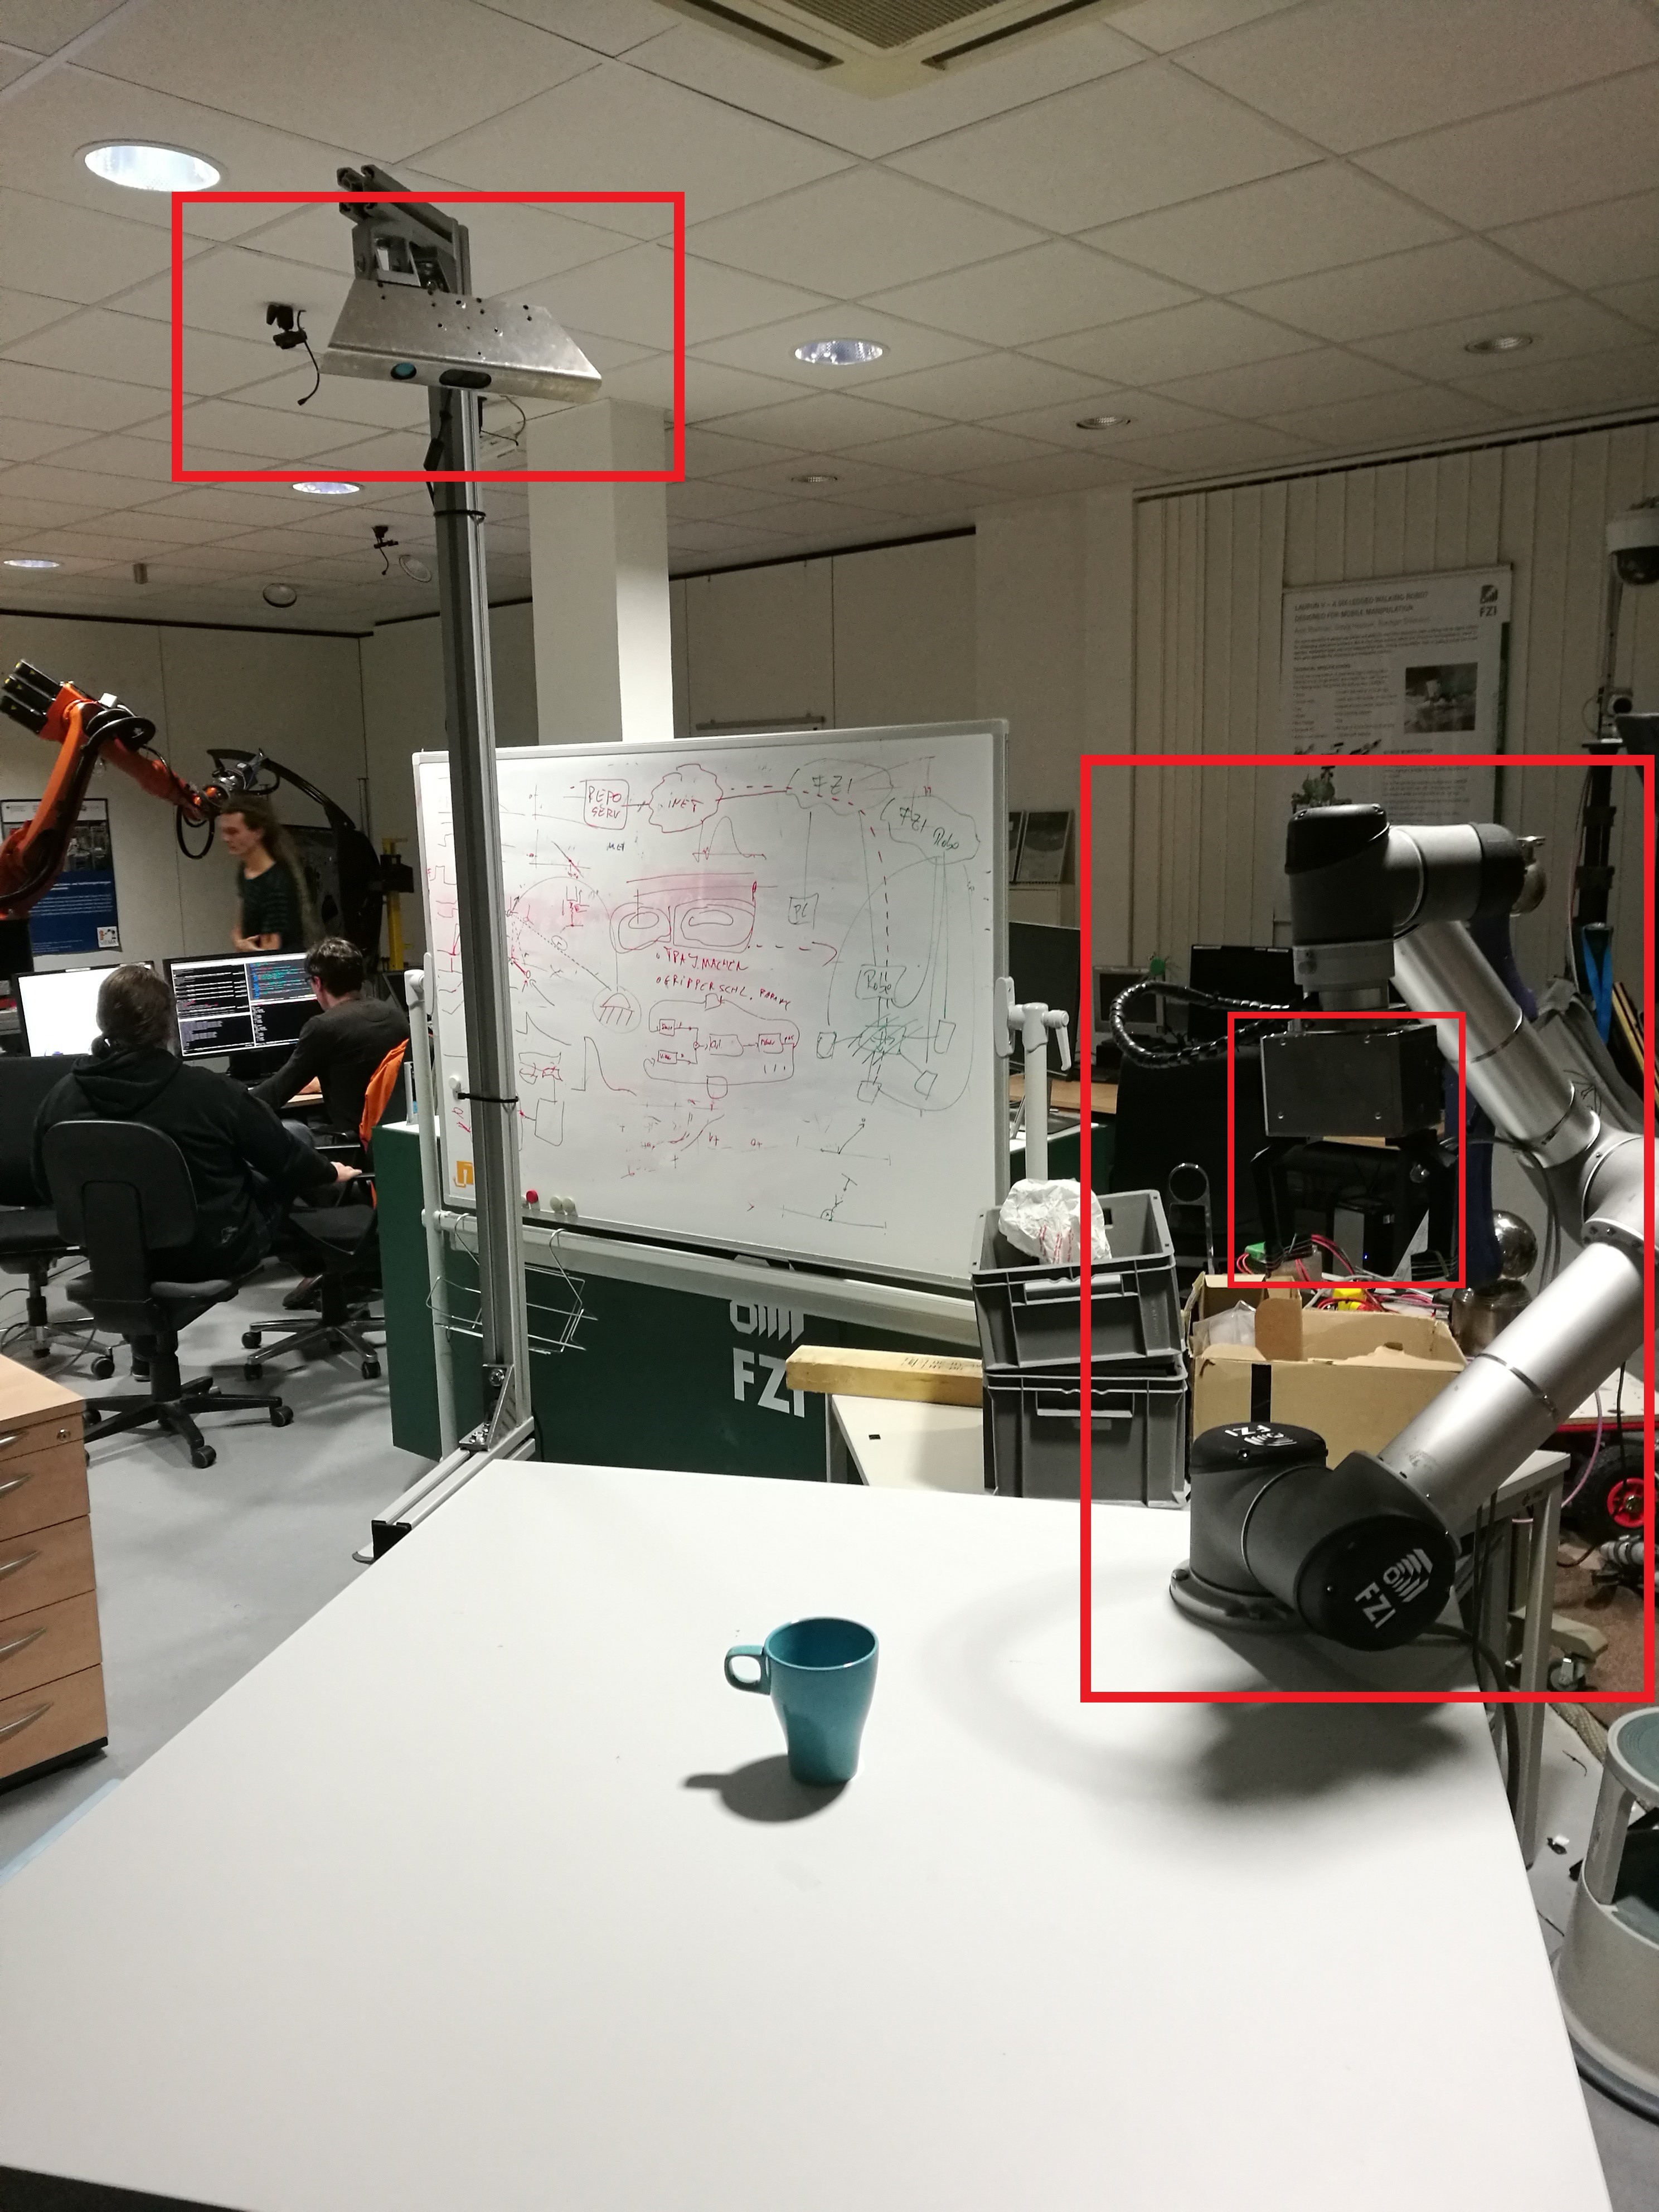
\includegraphics{images/Hardware-Aufbau.pdf}
	\caption{Aufbau der Hardware: Kinect Kamera (links oben), UR5 (rechts), PG70 (am Ende des UR5)}
	\label{Hardware}
\end{figure}